\documentclass{pptt}

\title{第十二届蓝桥杯省赛第一场题解}
\author{ACM算法与微应用开发实验室 \and AgOH}
\date{2022 年 1 月 29 日}

\begin{document}
\maketitle

\section{空间}

\begin{frame}{题面}
    小蓝准备用 256MB 的内存空间开一个数组,数组的每个元素都是 32 位二进制整数,如果不考虑程序占用的空间和维护内存需要的辅助空间,请问 256MB 的空间可以存储多少个 32 位二进制整数?
\end{frame}

\begin{frame}{题解}
    常识题,1MB=1024KB, 1KB=1024Bytes, 1Byte=8bits

    故 256MB 可以存储 $256 \times 1024 \times 1024 \times 8 \div 32=67108864$ 个 32 位二进制整数。

    答案:$67108864$
\end{frame}

\section{卡片}

\begin{frame}{题面}
    小蓝有很多数字卡片,每张卡片上都是数字 $0$ 到 $9$。

    小蓝准备用这些卡片来拼一些数,他想从 $1$ 开始拼出正整数,每拼一个,就保存起来,卡片就不能用来拼其它数了。

    小蓝想知道自己能从 $1$ 拼到多少。

    例如,当小蓝有 $30$ 张卡片,其中 $0$ 到 $9$ 各 $3$ 张,则小蓝可以拼出 $1$ 到 $10$,但是拼 $11$ 时卡片 $1$ 已经只有一张了,不够拼出 $11$。

    现在小蓝手里有 $0$ 到 $9$ 的卡片各 $2021$ 张,共 $20210$ 张,请问小蓝可以从 $1$ 拼到多少?
\end{frame}

\begin{frame}{题解}
    模拟即可,首先开一个数组 $a$,记录 $0 \sim 9$ 的卡片各有 $2021$ 张

    $i$ 从 $1$ 开始递增,对于每个 $i$,遍历其所有数位的数字,于数组 $a$ 中使卡片数量减 $1$,若发现无法减了(值为 $0$),则说明 $i$ 拼不出来,那么答案就是 $i-1$。

    答案:$3181$
\end{frame}

\section{直线}

\begin{frame}{题面}
    在平面直角坐标系中,两点可以确定一条直线。如果有多点在一条直线上,那么这些点中任意两点确定的直线是同一条。

    给定平面上 $2 \times 3$ 个整点 $\{(x,y)|0 \leq x < 2,~0 \leq y < 3,~x \in \mathbb{Z},~y \in \mathbb{Z}\}$,即横坐标是 $0$ 到 $1$ (包含 $0$ 和 $1$) 之间的整数、纵坐标是 $0$ 到 $2$(包含 $0$ 和 $2$)之间的整数的点。这些点一共确定了 $11$ 条不同的直线。

    给定平面上 $20 \times 21$ 个整点 $\{(x,y)|0 \leq x < 20,~0 \leq y < 21,~x \in \mathbb{Z},~y \in \mathbb{Z}\}$,即横坐标是 $0$ 到 $19$(包含 $0$ 和 $19$)之间的整数、纵坐标是 $0$ 到 $20$(包含 $0$ 和 $20$)之间的整数的点。请问这些点一共确定了多少条不同的直线。
\end{frame}

\begin{frame}{题解}
    我们只需要遍历所有点对,对于每对点对求出其所成直线的一般式(为什么是一般式?因为斜截式这种涉及到浮点数的方式,会因精度问题导致答案错误),然后装进 set 去重($Ax+By+C=0$ 只需要装 $(A,B,C)$ 即可),最后输出 set 的大小即可

    当然,因为一条直线有无限个一般式,所以不要忘记约分

    答案:$40257$
\end{frame}

\section{货物摆放}

\begin{frame}{题面}
    小蓝有一个超大的仓库,可以摆放很多货物。

    现在,小蓝有 $n$ 箱货物要摆放在仓库,每箱货物都是规则的正方体。小蓝规定了长、宽、高三个互相垂直的方向,每箱货物的边都必须严格平行于长、宽、高。

    小蓝希望所有的货物最终摆成一个大的立方体。即在长、宽、高的方向上分别堆 $L$、$W$、$H$ 的货物,满足 $n=L \times W \times H$。

    给定 $n$,请问有多少种堆放货物的方案满足要求。

    例如,当 $n=4$ 时,有以下 $6$ 种方案:$1 \times 1 \times 4$、$1 \times 2 \times 2$、$1 \times 4 \times 1$、$2 \times 1 \times 2$、$2 \times 2 \times 1$、$4 \times 1 \times 1$。

    请问,当 $n=2021041820210418$(注意有 $16$ 位数字)时,总共有多少种方案?
\end{frame}

\begin{frame}{枚举}
    直接暴力遍历 $L$ 和 $W$,$H$ 随之确定即可

    注意不是直接 $O(n^2)$ 暴力,$n=2021041820210418$,这属于作死

    容易发现,其实 $L$、$W$、$H$ 的组合只需要得出一次即可,因为三个数的其他组合可以靠组合数学解决:

    \begin{itemize}
        \item 若三个数互相不同,共有 $6$ 种排列方式
        \item 若只有两个数相同,共有 $3$ 种排列方式
        \item 若三个数相等,共有 $1$ 种排列方式
    \end{itemize}

    所以说 $L$ 只需要遍历到 $\sqrt[3]{n}$,$W$ 只需要遍历到 $\sqrt{\frac{n}{L}}$ 即可

    答案:$2430$
\end{frame}

\begin{frame}{质因数分解}
    首先找出 $2021041820210418$ 的质因子:

    $$2,3,3,3,17,131,2857,5882353$$

    然后问题就变成了把这 $8$ 个数分到三个集合(乘积分别作为 $L,W,H$)内且允许出现空集(视为 $1$)有几种方法。

    于是 $3^5 \times (1+3+6) = 2430$

    答案:$2430$
\end{frame}

\section{路径}

\begin{frame}{题面}
    小蓝学习了最短路径之后特别高兴,他定义了一个特别的图,希望找到图中的最短路径。

    小蓝的图由 $2021$ 个结点组成,依次编号 $1$ 至 $2021$。

    对于两个不同的结点 $a,b$,如果 $a$ 和 $b$ 的差的绝对值大于 $21$,则两个结点之间没有边相连;如果 $a$ 和 $b$ 的差的绝对值小于等于 $21$,则两个点之间有一条长度为 $a$ 和 $b$ 的最小公倍数的无向边相连。

    例如:结点 $1$ 和结点 $23$ 之间没有边相连;结点 $3$ 和结点 $24$ 之间有一条无向边,长度为 $24$;结点 $15$ 和结点 $25$ 之间有一条无向边,长度为 $75$。

    请计算,结点 $1$ 和结点 $2021$ 之间的最短路径长度是多少。
\end{frame}

\begin{frame}{题解}
    最短路裸题,因为没有负权边所以 Bellman-Ford,Dijkstra,甚至 Floyd 都行(反正是提答题)。

    答案:$10266837$
\end{frame}

\section{回路计数}

\begin{frame}{题面}
    蓝桥学院由 $21$ 栋教学楼组成,教学楼编号 $1$ 到 $21$。对于两栋教学楼 $a$ 和 $b$,当 $a$ 和 $b$ 互质时,$a$ 和 $b$ 之间有一条走廊直接相连,两个方向皆可通行,否则没有直接连接的走廊。

    小蓝现在在第一栋教学楼,他想要访问每栋教学楼正好一次,最终回到第一栋教学楼(即走一条哈密尔顿回路),请问他有多少种不同的访问方案?两个访问方案不同是指存在某个 $i$,小蓝在两个访问方法中访问完教学楼 $i$ 后访问了不同的教学楼。
\end{frame}

\begin{frame}{题解}
    dfs 爆搜时间复杂度过于巨大,显然不行。需要用状压 dp 来优化

    \begin{itemize}
        \item 设计状态:$dp[set][u]$ 代表当前到达点 $u$ 处且已经到达了 $set$ 中所有点的方案数($u \in set$)
        \item 初始状态:$dp[\{1\}][1]=1$
        \item 转移方程:$$dp[set][u]=\sum_{v \in set,(u,v) \in E}dp[set-u][v]$$
        \item 所求答案:$$\sum_{u \in V,(1,u) \in E}dp[V][u]$$
    \end{itemize}

    $set$ 为可用一二进制数 $s$ 表示(状态压缩),$s$ 的第 $i$ 位为 $1$ 代表 $i$ 结点已到达过

    答案:$881012367360$
\end{frame}

\section{时间显示}

\begin{frame}{题面}
    小蓝要和朋友合作开发一个时间显示的网站。在服务器上,朋友已经获取了当前的时间,用一个整数表示,值为从 $1970$ 年 $1$ 月 $1$ 日 $00:00:00$ 到当前时刻经过的毫秒数。

    现在,小蓝要在客户端显示出这个时间。小蓝不用显示出年月日,只需要显示出时分秒即可,毫秒也不用显示,直接舍去即可。

    给定一个用整数表示的时间,请将这个时间对应的时分秒输出。
\end{frame}

\begin{frame}{题解}
    题目给的输入即为毫秒级的 UNIX 时间戳,直接调库即可,注意需要输出 GMT 时间而不是 UTC 时间。

    \begin{itemize}
        \item \texttt{C/C++}:先把毫秒转化为秒,然后用 \texttt{gmtime} 转 \texttt{tm} 后再用 \texttt{strftime} 格式化输出。
        \item \texttt{Java}:\texttt{Date} 可以直接用毫秒时间戳构造,用 \texttt{SimpleDateFormat} 设置 GMT 时区后格式化输出。
        \item \texttt{Python}:先把毫秒转化为秒,\texttt{time.gmtime} 后 \texttt{time.strftime} 格式化输出。
    \end{itemize}

    当然不会调库的话也可以不调,因为只需要输出时分秒,所以把毫秒转换为秒后再对 $60 \times 60 \times 24=86400$ 取模,然后再转换出时分秒即可。
\end{frame}

\section{砝码称重}

\begin{frame}{题面}
    你有一架天平和 $N$ 个砝码,这 $N$ 个砝码重量依次是 $W_1,W_2,\cdots,W_N$。

    请你计算一共可以称出多少种不同的重量?

    注意砝码可以放在天平两边。
\end{frame}

\begin{frame}{题解}
    天平问题是经典的背包问题

    \begin{itemize}
        \item 设计状态:$dp[i][j]$ 表示选到第 $i$ 个砝码时重量 $j$ 能否称出来
        \item 初始状态:$dp[i][w_i]=true$
        \item 状态转移方程:$$dp[i][j]=dp[i-1][j] \lor dp[i-1][|j-w_i|] \lor dp[i-1][j+w[i]]$$
        \item 所求答案:$$\sum_{j=1}^{\sum w_i}[dp[n][j]=true]$$
    \end{itemize}

    第一维的转移只跟上一维有关,可以把式子拆开后使用滚动数组优化,不过在实现时要注意 $j$ 遍历的顺序

    $$dp[j]=dp[j] \lor dp[j-w_i],~dp[j]=dp[j] \lor dp[j+w_i]$$
\end{frame}

\section{杨辉三角形}

\begin{frame}{题面}
    下面的图形是著名的杨辉三角形:

    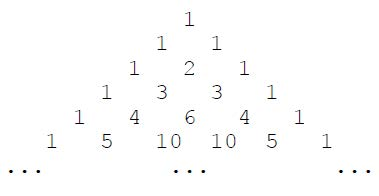
\includegraphics[scale=0.5]{images/yh.jpg}

    如果我们按从上到下、从左到右的顺序把所有数排成一列,可以得到如下数列:

    $1, 1, 1, 1, 2, 1, 1, 3, 3, 1, 1, 4, 6, 4, 1, \cdots$

    给定一个正整数 $N$,请你输出数列中第一次出现 $N$ 是在第几个数?
\end{frame}

\begin{frame}{题解}
    首先,本题一定有解,因为 $\dbinom{n}{1}=n$

    直接递推杨辉三角只能拿20分,空间及时间复杂度都太大了——都是 $O(n^2)$,我们需要分析一下

    显然杨辉三角形的右半部分是没用的,直接去掉即可

    对于杨辉三角中的任意一个数字,可以发现其必定大于其左上方的所有数字,也就是说我们可以把杨辉三角分成若干从右上到左下的斜列

    我们简单一些考虑,能递推出来的就暴力递推,不能递推出来的找规律算出来就是了:

\end{frame}

\begin{frame}
    \begin{itemize}
        \item 假设 $N$ 在第二斜列,那么显然最坏需要推 $N$ 层,不能承受,但显然第二斜列上数字对应行数,$N$ 即为数列的第 $\frac{N(N+1)}{2}+2$ 项
        \item 假设 $N$ 在第三斜列,那么最坏需要推 $\dbinom{r}{3} \leq {10}^9$ 解得 $r<=44722$ 层,还是不能承受。但我们发现第三斜列上的数字是逐行 $+4,+5,\cdots$ 的,所以一个循环遍历一下就好了
        \item 假设 $N$ 在第四斜列,那么最坏需要推 $\dbinom{r}{4} \leq {10}^9$ 解得 $r<=1819$ 层,这个是可以承受的,可以直接递推。另外显然第四斜列之后的斜列需要推的层数更少
    \end{itemize}

    所以我们的结题步骤即:首先递推出前 $1819$ 层,若发现 $N$ 则直接输出其位置。若没发现则遍历第三斜列。若还是没发现则答案为 $\frac{N(N+1)}{2}+2$。
\end{frame}

\section{双向排序}

\begin{frame}{题面}
    给定序列 $(a_1,a_2,\cdots,a_n) = (1,2,\cdots,n)$,即 $a_i=i$。

    小蓝将对这个序列进行 $m$ 次操作,每次可能是将 $a_1,a_2,\cdots,a_{q_i}$ 降序排列,或者将 $a_{q_i},a_{q_i+1},\cdots,a_n$ 升序排列。

    请求出操作完成后的序列。
\end{frame}

\begin{frame}{栈}
    直接暴力排序的时间复杂度为 $O(mn\log{n})$ 的,只能得到 $60$ 分。

    我们可以发现,对于连续的几条同一种操作,显然覆盖范围最广的会覆盖掉其它操作,所以首先我们使用一个栈来维护操作,使得两种操作在栈内交替出现

    然后,对于每个操作:

    \begin{itemize}
        \item 若该操作与上一条操作的覆盖范围不相交,则该操作无效
        \item 若该操作与上一条操作的覆盖范围相交,那么:
              \begin{itemize}
                  \item 若相交的范围在上一对操作的相交范围之内,则对相交部分进行翻转即可
                  \item 若相交的范围不在上一对操作的相交范围之内,则上一对操作无效
              \end{itemize}
    \end{itemize}

    可以发现我们需要做的事情只有不停的翻转某区间,而且需要翻转的区间是在不停变小的,所以说范围外的值一旦确定就不会更改,直接填数就好了

    时间复杂度 $O(n+m)$
\end{frame}

\begin{frame}{线段树分裂合并}
    本题为 \texttt{[HEOI2016/TJOI2016]排序} 的弱化版,故解决方法相同:线段树分裂合并。

    \begin{center}
        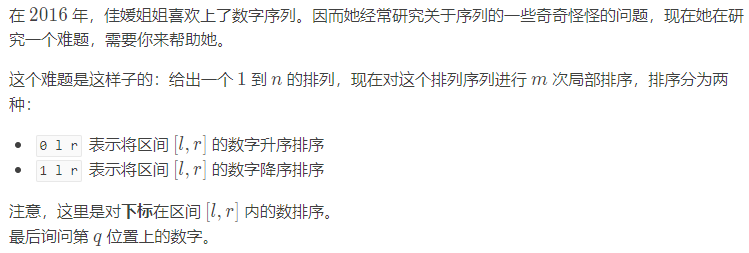
\includegraphics[scale=0.4]{images/sort.png}
    \end{center}

    因为值域线段树上的数是有序的,故对于排序操作即通过线段树的分裂合并操作使用一个值域线段树维护操作区间即可。

    时间复杂度 $O(m\log{n})$
\end{frame}

\section{异或数列}

\begin{frame}{题面}
    \texttt{Alice} 和 \texttt{Bob} 正在玩一个异或数列的游戏。初始时,\texttt{Alice} 和 \texttt{Bob} 分别有一个整数 $a$ 和 $b$,有一个给定的长度为 $n$ 的公共数列 $X_1,X_2,\cdots,X_n$。

    \texttt{Alice} 和 \texttt{Bob} 轮流操作,\texttt{Alice} 先手,每步可以在以下两种选项中选一种:

    \begin{itemize}
        \item 选项1:从数列中选一个 $X_i$ 给 \texttt{Alice} 的数异或上,或者说令 $a$ 变为 $a \oplus X_i$。(其中 $\oplus$ 表示按位异或)
        \item 选项2:从数列中选一个 $X_i$ 给 \texttt{Bob} 的数异或上,或者说令 $b$ 变为 $b \oplus X_i$。
    \end{itemize}

    每个数 $X_i$ 都只能用一次,当所有 $X_i$ 均被使用后($n$ 轮后)游戏结束。游戏结束时,拥有的数比较大的一方获胜,如果双方数值相同,即为平手。

    现在双方都足够聪明,都采用最优策略,请问谁能获胜?
\end{frame}

\begin{frame}{题解}
    因为是最后剩下的数字比较大的一方获胜,所以我们只需要从高到低考虑每个二进制位即可:如果某个二进制位上已经可以决出胜负,则结束;如果每一位都是平局则平局

    对于所有数字的某位:

    \begin{itemize}
        \item 若 $1$ 的数量为偶数(包括 $0$ 个),因为所有的 $1$ 都要用上,所以必定平局;
        \item 若 $1$ 的数量为奇数且没有 $0$,因为当 $1$ 的数量为偶数时必定平局,所以当 $1$ 的数量为奇数时因为该先手方进行操作故先手方只需要给自己异或 $1$ 即可必胜。
        \item 若有 $0$ 的存在,因为 $0$ 异或一个数结果还是这个数所以选择用 $0$ 异或相当于换手
              \begin{itemize}
                  \item 若 $0$ 的数量为偶数,因为所有 $0$ 都要用上,所以相当于没有 $0$(换手再换手等于没换)
                  \item 若 $0$ 的数量为奇数,相当于只有 $1$ 个 $0$
                        \begin{itemize}
                            \item 若 $1$ 的数量为 $1$,先手方只需要给自己异或上 $1$ 即可胜出
                            \item 若 $1$ 的数量为 $3,5,7,\cdots$,因为 $0$ 的存在导致后手方可以变为先手,所以本来的先手必胜变成了后手必胜
                        \end{itemize}
              \end{itemize}
    \end{itemize}

    为什么当 $0$ 的数量为奇数 $1$ 的数量为 $1$ 时同样是奇数却是先手必胜呢?因为后手方利用换手获胜的必要条件是换手后还有 $1$ 进行操作,而 $1$ 的数量为 $1$ 时先手方给自己异或上 $1$ 后导致没有剩余的 $1$ 进行操作了,后手方的换手就变成了无用之举
\end{frame}

\section{左孩子右兄弟}

\begin{frame}{题面}
    对于一棵多叉树,我们可以通过“左孩子右兄弟” 表示法,将其转化成一棵二叉树。

    如果我们认为每个结点的子结点是无序的,那么得到的二叉树可能不唯一。换句话说,每个结点可以选任意子结点作为左孩子,并按任意顺序连接右兄弟。

    给定一棵包含 $N$ 个结点的多叉树,结点从 $1$ 至 $N$ 编号,其中 $1$ 号结点是根,每个结点的父结点的编号比自己的编号小。请你计算其通过“左孩子右兄弟” 表示法转化成的二叉树,高度最高是多少。注:只有根结点这一个结点的树高度为 $0$。
\end{frame}

\begin{frame}
    例如如下的多叉树: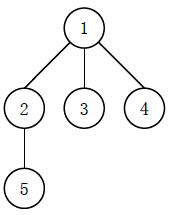
\includegraphics[scale=0.4]{images/1.jpg}

    可能有以下 3 种(这里只列出 3 种,并不是全部)不同的“左孩子右兄弟”表示:

    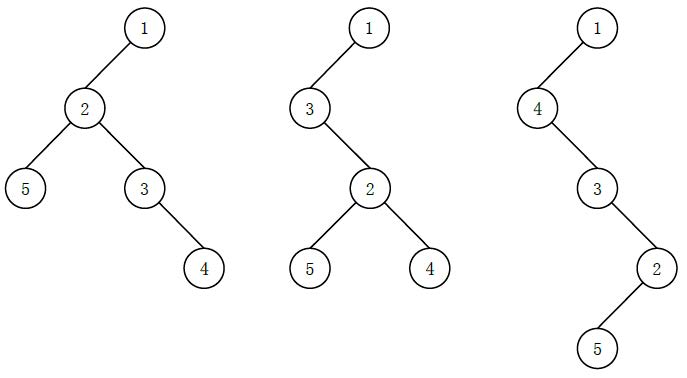
\includegraphics[scale=0.4]{images/2.jpg}

    其中最后一种高度最高,为 $4$。
\end{frame}

\begin{frame}{题解}
    显然对于一个结点我们只需要贪心地把其高度最高的子树尽量往下挂即可,极为简单的一道树上 DP

    \begin{itemize}
        \item 状态设计:$dp[u]$ 代表 $u$ 结点对高度的最大贡献
        \item 初始状态:$dp[leaf]=0$
        \item 状态转移:$$dp[u]=son[u].length + \max_{v \in son[u]}dp[v]$$
        \item 所求答案:$dp[rt]$
    \end{itemize}
\end{frame}

\section{括号序列}

\begin{frame}{题面}
    给定一个括号序列,要求尽可能少地添加若干括号使得括号序列变得合法,当添加完成后,会产生不同的添加结果,请问有多少种本质不同的添加结果。两个结果是本质不同的是指存在某个位置一个结果是左括号,而另一个是右括号。

    例如,对于括号序列 \texttt{((()},只需要添加两个括号就能让其合法,有以下几种不同的添加结果:\texttt{()()()}、\texttt{()(())}、\texttt{(())()}、\texttt{(()())} 和 \texttt{((()))}。
\end{frame}

\begin{frame}{题解}
    因为尽可能添加少的括号,所以添加的左、右括号不会出现如同 \texttt{()} 的形式,所以左括号与右括号添加的位置方案是相互独立的,不会相互影响。故总的方案数等于左括号的方案数 $\times$ 右括号的方案数。继续转换成只需要添加左括号:当需要添加右括号时将整个括号序列对称翻转,就转化为只需要添加左括号了

    若以右括号为分割点将整个序列进行分割,因为分割后的子串中均为左括号,添加任意数目的左括号方案数均为一种,那么此时我们仅需考虑添加不同数量的左括号的方案数即可。采用 DP:

    设 $n$ 为右括号数,$x$ 为共需添加多少个左括号,$b$ 代表当前至少需添加多少个左括号

    \begin{itemize}
        \item 状态设计:$dp[i][j]$ 代表只考虑前 $i$ 个右括号,需要添加 $j$ 个左括号的方案数
        \item 初始状态:$dp[1][~]=1$
        \item 状态转移:$$dp[i][j]=\sum_{k=b}^{x}dp[i-1][k]$$
        \item 所求结果:$dp[n][x]$
    \end{itemize}
\end{frame}

\end{document}
